%% 内容梗概

%% プリアンブル %%%%%%%%%%%%%%%%%%%%%%%%%%%%%%%%%%%%%%%%%%%%%%%%%%%%%%%%
\documentclass[a4j,dvipdfmx]{jarticle}

\usepackage{kut-abstract}  
\usepackage{url}
\usepackage{enumitem}
\usepackage{booktabs}
\usepackage{amssymb}
\usepackage{tikz}
\usepackage{adjustbox} % preamble に追加
\usepackage{tabularx, booktabs}
\usepackage{float}

\newcolumntype{Y}{>{\raggedright\arraybackslash}X}

\usetikzlibrary{arrows.meta}
\setlist[itemize]{noitemsep, parsep=0pt, partopsep=0pt}

%% 表題 %%%%%%%%%%%%%%%%%%%%%%%%%%%%%%%%%%%%%%%%%%%%%%%%%%%%%%%%%%%%%%%%
%% 注意! 情報学群生の場合は，以下の \ScInfo を有効にすること．
% \ScInfo        %% 情報学群生の場合

% \Bachelor	%% 卒業研究論文梗概の場合
% \Project	%% プロジェクト研究報告書梗概の場合
%\Seminar	%% 特別研究セミナー課題研究報告書梗概の場合
%\Master	%% 修士学位論文（情報システム工学コース）梗概の場合
%\Doctorate	%% 博士学位論文（情報システム工学コース）梗概の場合
%\English	%% 英語の場合

% \Eyears{2006}
% \Etitle{English Title}
% %\idnumber{}
% \Eauthor{HASHIMOTO, Manabu}
% \Eaffiliate{Sakamoto Lab.}

%% 本文 %%%%%%%%%%%%%%%%%%%%%%%%%%%%%%%%%%%%%%%%%%%%%%%%%%%%%%%%%%%%%%%%

\title{大貧民におけるグラフニューラルネットワークを用いた評価関数の設計・評価 \\
\vspace{0.3em}
\large Design and Evaluation of Evaluation Function \\ Using Graph Neural Network in Daihinmin}
\idnumber{}
\author{福澤 詩音   ~~~ 松崎 公紀 ~~~~}
\affiliate{高知工科大学}
%% 本文 %%%%%%%%%%%%%%%%%%%%%%%%%%%%%%%%%%%%%%%%%%%%%%%%%%%%%%%%%%%%%%%%
\begin{document}
\begin{Abstract}
 
 \section{はじめに}
大貧民は日本で広く親しまれているトランプゲームであり，多人数・不完全情報ゲームに分類される．
ペアや階段といった役，8切りや革命による強弱の反転などの独自ルールを持ち，
相手の手札や戦略を読みながら自分の手札を効率よく処理する戦略性が求められる．
大貧民は，UECコンピュータ大貧民大会(UECda)~\cite{bib:uecdda}を中心に研究が進められ，
探索を用いたプレイヤが長く上位を占めてきた~\cite{bib:ohto2016}．
しかし，純粋なNN評価関数のみで探索プレイヤを凌駕するクライアントは存在しない．

本研究では，探索を用いないニューラルネットワーク型評価関数を設計し，その有効性を検証する．
特に，局面をカードのグラフとして表現するグラフニューラルネットワーク型の評価関数を提案し，
局面を画像として捉える畳み込みニューラルネットワーク，および両者の特徴を融合したモデルと
比較して評価実験を行う．

大貧民では，手札中の一枚のカードが複数の役に同時に属しうるため，候補手は互いに独立ではない．
ある候補手を選択すると，そのカードを共有する他の候補手は以後提出不可能となる．
したがって着手選択は，その場で得られる利得と，将来の強力な役を温存することによる期待利得とのトレードオフを含む問題となる．

そのため，カードと提出手の関係をグラフで明示的に表現することが可能なGNNは，大貧民の評価関数設計に適していると考えた．

グラフニューラルネットワーク(GNN)は,グラフ構造データを入力し,隣接ノードの特徴を集約してノードやグラフ全体の表現を学習する.
代表的手法のGCN~\cite{bib:gcn}は文献ネットワークのノード分類で高精度を示した.
ゲーム研究にも応用され,チェスをノードと指し手のグラフで表現しGNNで評価関数を学習する研究~\cite{bib:alphagateau}があるが,依然として研究例は少ない．



\section{大貧民のグラフ表現}
図\ref{fig:graph_examples}に，大貧民の各局面の状態をグラフで表現した例を示す．一つ目は，ゲームで用いる53枚のカードをノードとするグラフである（表\ref{tab:graph_card}）．
同じランクのカード同士を無向辺で結び，さらに強さが隣り合うカードを弱い方から強い方へ向かう有向辺で結ぶことで，カードの強弱の順序を表現する．革命によって強弱が反転した場合は，この強さ方向の辺の向きを逆にすることで盤面の変化を反映する．

二つ目は，自身の手札のカードと，そこから構成される候補手とを結ぶ
二部グラフである（表\ref{tab:graph_bipartite}）．候補手とは場の状況において提出可能な一つ一つの手であり，各候補手のノードはそれを構成するカードのノードと辺で結ばれる．
これにより一つ目のグラフで得たカードの表現を集約して候補手の表現を作り，どのカードの組み合わせがどの手に対応するのかをネットワークへ与える．

\begin{table}[t]
  \centering
  \caption{カードグラフの仕様}
  \label{tab:graph_card}
  \small
  \begin{tabularx}{0.85\linewidth}{l >{\raggedright\arraybackslash}X}
    \toprule
    項目 & 内容 \\
    \midrule
    ノード       & 53枚のカード \\
    ノードの特徴 & スート，ランク，強さ，手札か否か，捨て札 \\
    辺           & 同ランク辺（無向），強さ順辺（有向，革命で反転） \\
    辺の範囲     & 手札のカード間のみ \\
    処理         & 多関係グラフ畳み込み（4層） \\
    \bottomrule
  \end{tabularx}
\end{table}

\begin{table}[t]
  \centering
  \caption{手札カードと役の二部グラフの仕様．}
  \label{tab:graph_bipartite}
  \small
  \begin{tabularx}{0.85\linewidth}{l >{\raggedright\arraybackslash}X}
    \toprule
    項目 & 内容 \\
    \midrule
    ノード       & 手札カードと役（候補手） \\
    ノードの特徴 & 役：構成カードの平均，手のタイプ，枚数 \\
    辺           & 手札カード $\rightarrow$ 役（構成関係） \\
    辺の範囲     & 手札カードとそれが作る役の間 \\
    処理         & 構成カードを集約して役を表現 \\
    \bottomrule
  \end{tabularx}
\end{table}

\begin{figure}[t!]
  \centering
  \begin{minipage}{0.48\linewidth}
    \centering
    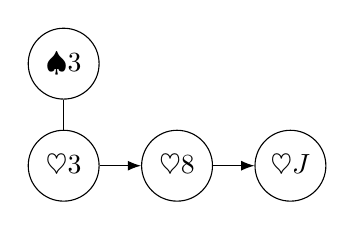
\begin{tikzpicture}[>=Latex,scale=0.72]
      \tikzset{card/.style={circle,draw,minimum size=9mm,inner sep=1pt}}
      \node[card] (s3) at (0,0) {$\spadesuit 3$};
      \node[card] (h3) at (0,-1.8) {$\heartsuit 3$};
      \node[card] (h8) at (2,-1.8) {$\heartsuit 8$};
      \node[card] (hj) at (4,-1.8) {$\heartsuit J$};

      \draw (h3) -- (s3);
      \draw[->] (h3) -- (h8);
      \draw[->] (h8) -- (hj);
    \end{tikzpicture}
    \\ \footnotesize (a) カードグラフの例
  \end{minipage}
  \hfill
  \begin{minipage}{0.48\linewidth}
    \centering
    \begin{tikzpicture}[>=Latex,scale=0.72]
      \tikzset{
        card/.style={circle,draw,minimum size=7mm,inner sep=0.5pt,font=\small},
        move/.style={rounded corners=2pt,draw,minimum width=18mm,minimum height=3mm,inner sep=1pt,font=\small}
      }
      \node[card] (h3) at (0,0.8) {$\heartsuit 3$};
      \node[card] (s3) at (0,-0.2) {$\spadesuit 3$};
      \node[card] (h8) at (0,-1.3) {$\heartsuit 8$};

      \node[move] (m33) at (3.2,1.0) {$3$ のペア};
      \node[move] (mh3)  at (3.2,0.5) {$\heartsuit 3$ 単体};
      \node[move] (ms3)  at (3.2,0.0) {$\spadesuit 3$ 単体};
      \node[move] (mh8)  at (3.2,-1.3) {$\heartsuit 8$ 単体};

      \draw[->] (h3.east) -- (m33.west);
      \draw[->] (h3.east) -- (mh3.west);
      \draw[->] (s3.east) -- (ms3.west);
      \draw[->] (s3.east) -- (m33.west);
      \draw[->] (h8.east) -- (mh8.west);
    \end{tikzpicture}
    \\ \footnotesize (b) 二部グラフの例
  \end{minipage}
  \caption{大貧民のグラフ表現の例}
  \label{fig:graph_examples}
\end{figure}

 \section{実験}
本研究で比較するモデルは以下の3つである．
\vspace{-2mm}
\begin{itemize}
  \item GNN：隠れ次元は128，カード埋め込みは64次元とし，同ランク辺・強さ順辺・自己ループの各経路を集約する．
  \item CNN：盤面を4×13の画像として扱う畳み込みネットワークであり，残差ブロック（ResNet型）を積む．
  \item 融合：学習済みの GNN と CNN が出力する候補手表現および文脈を連結し，共通の全結合ヘッドで方策と状態価値を出力する．
\end{itemize}
\vspace{-2mm}
教師データにはUECdaコンピュータ大貧民大会に出場したクライアントの指し手を用いた．具体的にはBlauweregenと他の出場クライアントであるjn17，res.kou2，GAM，switch，Rappa，Ganesa，大会サンプルエージェントを対戦させ，Blauweregenが選択した手を教師データとして抽出した．
試合数は10万試合，局面数にして114万局面であり，学習データと検証データに8:2の割合で分割した．

学習は，候補手の中から Blauweregen が選んだ手を当てる教師あり学習で行う．損失は方策の交差エントロピーと状態価値の二乗誤差の和とした．最適化には Adam を用い，学習率は $1\times10^{-4}$ を初期値として設定し，エポック数は30とした．

評価は，学習したモデルを1体，公開クライアント switch を相手4体として4000局対戦させ，平均得点で比較した．

各モデルの switch 4体との対戦成績を表\ref{tab:result}に示す．
switch 4体の合計スコアがおよそ12000台であるのに対し，GNNは10680，CNNは10400，
融合モデルは11360であり，いずれも上回らなかった．CNNとGNNに明確な差は見られなかったが，融合モデルは単体よりも高いスコアを示した．

図\ref{fig:accuracy}に，各モデルの方策損失と価値損失の推移を示す．方策・価値損失ともにCNNが最も大きく，次点でGNN，最も小さいのが融合モデルであった．CNNは15エポック目以降に方策損失が増加しているが，GNNや融合モデルではそのような傾向は見られず，学習が安定していることが分かる．価値損失は，全モデルとも学習が進むにつれ減少していた．

表\ref{tab:acc}の各列は以下を表す．
一致率は，モデルが最も高いスコアを与えた手が教師の選択した手と一致した局面の割合である．
非自明一致率は，提出可能な候補手が3つ以上存在する局面に限定した一致率であり，
パスや提出可能な手が1つのみといった選択の余地が小さい局面を除いた，
より判断を要する局面での精度を表す．
選択確率は，モデルが出力する各手の確率のうち，教師が実際に選択した手へ与えた確率の平均であり，
値が大きいほど教師の手を高い確信度で予測していることを示す．
価値MSEは，各局面の価値の予測値と，その局を最後までプレイした際に実際に得られた
正規化報酬との平均二乗誤差であり，値が小さいほど盤面の有利不利を正確に予測できていることを示す．

\section{考察}
融合が単体および出力平均を上回った要因として，GNN と CNN の相補性が挙げられる．同一局面での両者の選択を比較すると，約2割の局面で判断が分かれ，GNN は保守的に札を温存し弱い札を出す傾向を，CNN は強い札を切る攻撃的な傾向を示した．異なる観点で盤面を捉える二つのモデルを特徴レベルで統合することで，一方だけでは得られない判断が可能になったと考えられる．学習時の損失でも，融合は方策と価値の双方が最も低く収束したのに対し，CNN 単体は途中から方策の損失が増加し過学習の傾向を示した．

負けた対局を分析すると，その多くは配牌が弱く打開が困難な局面であった．一方で，一度優勢になりながら終盤で順位を落とす対局も一定数見られ，多手先の手順を要する終盤の詰めに課題があることが分かった．これは各局面での手の予測にとどまり，多手先を読む探索を備えていないことに起因すると考えられる．


\begin{table}[t]
  \centering
  \caption{switch 4体との対戦成績（4000局）}
  \label{tab:result}
  \small
  \begin{tabular}{lrr}
    \toprule
    モデル & 最終スコア & 平均得点 \\
    \midrule
    GNN & 10680 & 2.67 \\
    CNN & 10400 & 2.60 \\
    \textbf{CNN ＋ GNN} & \textbf{11360} & \textbf{2.84} \\
    \bottomrule
  \end{tabular}
% \end{table}

% \begin{table}[t]
  \centering
  \caption{各モデルの一致率と価値予測精度}
  \label{tab:acc}
  \begin{tabular}{lcccc}
    \hline
    モデル & 一致率 & 非自明一致率 & 選択確率 & 価値MSE \\
    \hline
    融合   & \textbf{0.774} & \textbf{0.718} & \textbf{0.725} & \textbf{0.103} \\
    GNN    & 0.762 & 0.707 & 0.690 & 0.104 \\
    CNN    & 0.762 & 0.702 & 0.699 & 0.119 \\
    \hline
  \end{tabular}
\end{table}

\begin{figure}[t]
  \centering
  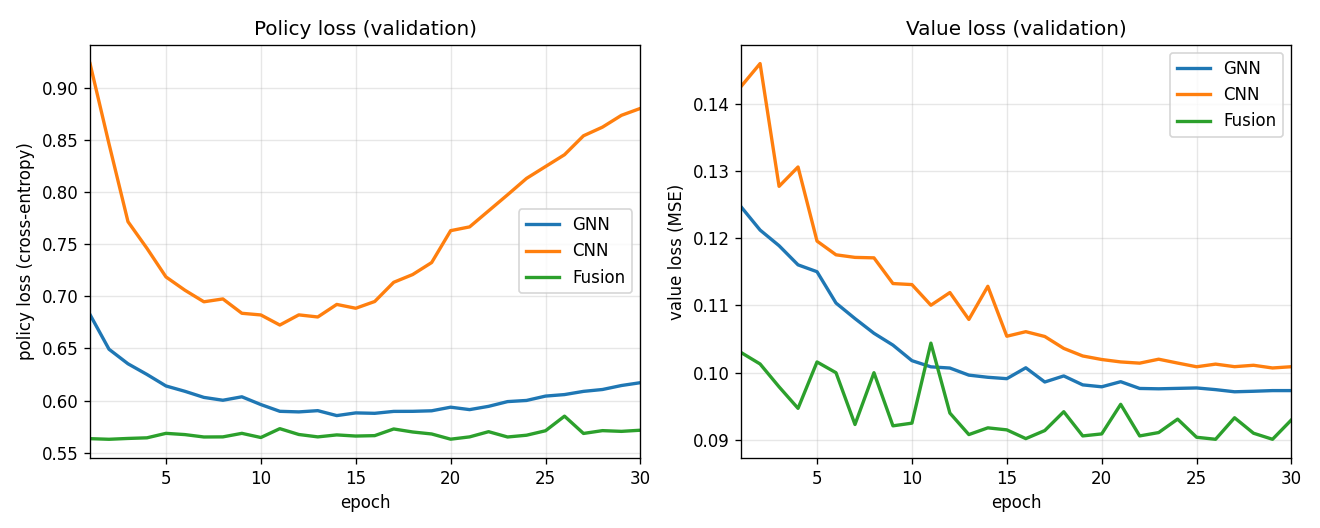
\includegraphics[trim=0mm 0mm 0mm 15mm, clip,width=\linewidth]{figure/loss_overlay_all.png}
  \caption{各モデルの方策・価値損失の推移}
  \label{fig:accuracy}
\end{figure}

\section{まとめ}
本研究では，大貧民の局面をカード間の関係を表すグラフと，
手札と候補手を結ぶ二部グラフの二つで表現し，
グラフニューラルネットワークにより方策と状態価値を学習する手法を提案した．
GNN，CNN，および両者を結合する融合モデルを比較した結果，
融合モデルが一致率と価値予測精度のいずれでも最も高い性能を示した．
本稿では，敗因のさらに具体的な分析を進める．
%% 参考文献 %%%%%%%%%%%%%%%%%%%%%%%%%%%%%%%%%%%%%%%%%%%%%%%%%%%%%%%%%%%%
\begin{thebibliography}{99}\small
 \bibitem{bib:uecdda}電気通信大学,
         ``UECdaコンピュータ大貧民大会'',
         \url{https://flute.u-shizuoka-ken.ac.jp/daihinmin/2023/document_rules.html}，2026年7月閲覧.

\bibitem{bib:alphagateau} Tomas Rigaux, Hisashi Kashima, ``Enhancing Chess Reinforcement Learning with Graph Representation'', 38th Conference on Neural Information Processing Systems NeurIPS 2024.

\bibitem{bib:gcn} Thomas N. Kipf, Max Welling, ``Semi-Supervised Classification with Graph Convolutional Networks'', Published as a conference paper at ICLR 2017.

\bibitem{bib:ohto2016} 大渡勝己, 田中哲朗, ``方策勾配を用いた教師有り学習によるコンピュータ大貧民の方策関数の学習とモンテカルロシミュレーションへの利用'', 情報処理学会研究報告, 2016.


  
\end{thebibliography}

\end{Abstract}
\end{document}